\documentclass[a4paper]{article}

% Packages
\usepackage[utf8]{inputenc}
\usepackage[top=50pt,bottom=60pt,left=1in,right=1in]{geometry}
\usepackage{natbib}
\usepackage{graphicx}


%% These few lines make a distinction between latex and pdflatex calls and they
%% bring in essential packages for graphics and font handling.
%% Note that due to the \DeclareGraphicsExtensions{} call it is no longer necessary
%% to provide the the path and extension of a graphics file:
%% 
\includegraphics{diamondrule} is completely sufficient.
%%
\ifpdf%                                % if we use pdflatex
  \pdfoutput=1\relax                   % create PDFs from pdfLaTeX
  \pdfcompresslevel=9                  % PDF Compression
  \pdfoptionpdfminorversion=7          % create PDF 1.7
  \ExecuteOptions{pdftex}
  \usepackage{graphicx}                % allow us to embed graphics files
  \DeclareGraphicsExtensions{.pdf,.png,.jpg,.jpeg} % for pdflatex we expect .pdf, .png, or .jpg files
\else%                                 % else we use pure latex
  \ExecuteOptions{dvips}
  \usepackage{graphicx}                % allow us to embed graphics files
  \DeclareGraphicsExtensions{.eps}     % for pure latex we expect eps files
\fi%

\graphicspath{{figures/}{pictures/}{images/}{./}} % where to search for the images

\usepackage{microtype}                 % use micro-typography (slightly more compact, better to read)
\PassOptionsToPackage{warn}{textcomp}  % to address font issues with \textrightarrow
\usepackage{textcomp}                  % use better special symbols
\usepackage{mathptmx}                  % use matching math font
\usepackage{times}                     % we use Times as the main font
\renewcommand*\ttdefault{txtt}         % a nicer typewriter font
\usepackage{hyperref}                  % to enable \autoref
\usepackage{subcaption}                % to support captions for subfigures
\usepackage{enumitem}
\usepackage{physics}

% Title
\title{Volume Rendering Assignment\\2IMV20\\Eindhoven University of Technology}

% Authors and group. Replace with your names and group number
\author{Nimo Beeren \quad Henrique Dias \quad Gabriela Slavova\\Group 13}
\date{December 2020}

% Begin document
\begin{document}

\maketitle

\section{Introduction}

In class, various rendering methods used to visualize 3D scalar data have been discussed \citep{2imv20_2}. In this report, we describe our implementation of some of these methods and compare them by applying them to various datasets.

Each section contains a reference to the method where the implementation can be found. Unless otherwise mentioned, these methods are members of the {\tt RaycastRenderer} class.

\section{Implementation}

\subsection{Raycasting}
\label{subsec:raycasting}

\paragraph{Trilinear interpolation}

In order to achieve a smooth transition of intensity between voxels, we apply some interpolation. Given a 3D pixel coordinate $X$, we find the voxels $X_0 \ldots X_7$ such that these voxels form the vertices of a cube that contains $X$. Using the known intensities $S_{X_0}\ldots S_{X_7}$, we apply trilinear interpolation to obtain an approximate intensity for the given pixel coordinate:
\begin{align*}
  S_X =\;&(1 - \alpha) (1 - \beta) (1 - \gamma) S_{X_0}
    + \alpha (1 - \beta) (1 - \gamma) S_{X_1}\\
    &+ (1 - \alpha) \beta (1 - \gamma) S_{X_2}
    + \alpha \beta (1 - \gamma) S_{X_3}\\
    &+ (1 - \alpha) (1 - \beta) \gamma S_{X_4}
    + \alpha (1 - \beta) \gamma S_{X_5}\\
    &+ (1 - \alpha) \beta \gamma S_{X_6}
    + \alpha \beta \gamma S_{X_7}
\end{align*}
We expect that the visualization of the data after trilinear interpolation is implemented will be smoother and this can be observed in \autoref{fig:trilinear}. The implementation can be found in the method {\tt getVoxelTrilinear}.

\paragraph{Compositing}
\label{ray_composite}

To implement the compositing ray function, we applied a front-to-back compositing strategy, similar to the back-to-front strategy studied in class \citep{2imv20_2}:
$$I(p)=\sum^{n-1}_{i=0}c_i\prod^{n-1}_{j=i+1}(1-\alpha_j)$$
where $\alpha_j$ is the voxel opacity and $c_i$ the color. Since this calculation is based on a sum, we calculate it iteratively. Using the given {\tt rayVector} and {\tt sampleStep} values, we can calculate the incremental step to go from {\tt entryPoint} to {\tt exitPoint}. For each voxel, we calculate the value using trilinear interpolation and the trilinear gradient and add it to the final voxel color. The implementation can be found in the method {\tt traceRayComposite}.

\paragraph{Interactive mode}
\label{speed_up}

To make the application more responsive while manipulating the camera, we lower the resolution during rendering. We can do that by changing the values of the variables {\tt increment} and {\tt sampleStep} to bigger ones leading to lowering the number of steps along the view ray and the number of pixels sampled.  The new values for interactive mode were chosen using the trial-and-error method to find a workable trade-off between rendering quality and performance. In \autoref{fig:speedup} can be observed both the time of the rendering in interactive mode before and after the changes, and the the quality of the image. The implementation consists of a simple if-statement near the top of the {\tt raycast} method.

\paragraph{Gradients}
\label{subsec:gradients}

The work related to gradients consists of two main parts:

\begin{enumerate}[noitemsep]
  \item Computing the gradients, implemented in method {\tt compute} of class {\tt GradientVolume}.
  \item Trilinear interpolation of gradients, implemented in method {\tt getGradientTrilinear}.
\end{enumerate}

\noindent When the volume is first loaded, an approximate gradient is computed for all voxels, using the method described by Levoy \citep{levoy_1988}. The resulting vectors are stored in a lookup table (LUT).

To achieve a smooth transition of the gradient between voxels, we apply trilinear interpolation in similar fashion as done with the voxel intensities. To aid with scalar multiplication and vector addition, the utility methods {\tt scale} and {\tt add} respectively were implemented in the {\tt VoxelGradient} class.

\subsection{Isosurface raycasting and shading}
\label{subsec:isosurface}

\paragraph{Isosurface raycasting}

Isosurfaces are defined by
 $$f(x; y; z) = C$$ 
Where $C$ is a constant known as the isovalue. Similarly to the compositing method described in \autoref{subsec:raycasting}, we use the given {\tt rayVector} and {\tt sampleStep} values to calculate the incremental step to go from {\tt entryPoint} to {\tt exitPoint}. For each voxel, we use trilinear interpolation to calculate the value and then we compare it to the value of {\tt isoValueFront} which is the value specified in the GUI of the application. If the current value is greater we check if shading is enabled and apply it using {\tt computePhongShading} if needed, and return the {\tt isoColorFront} which is the chosen color in the GUI of the application or the newly computed color after the shading is applied to the  {\tt isoColorFront}. If no greater than {\tt isoValueFront} values are found, black is returned.

After implementation we should be able to clearly see parts with the same value. The result without shading enabled can be seen in \autoref{fig:isosurface}. Rendering using this method is fast and does not cause any delays in the interaction with the GUI. The implementation can be found in the method {\tt traceRayIso}.

\paragraph{Phong shading}

Phong's shading model was presented in class \citep{2imv20_2}:

$$I = I_a k_a + I_l k_d(L \cdot N) + I_l k_s(V \cdot R)^\alpha$$

\noindent where

\begin{itemize}
  \item $I_a$ and $I_l$ are the color of the ambient light and the direct light, respectively.
  \item $k_a$, $k_d$ and $k_s$ are the ambient, diffuse and specular parameters, respectively.
  \item $L$ is the light vector, pointing towards the light source.
  \item $N$ is the normal vector which can be approxmiated by $N = {G}/{|G|}$ where $G$ is the local gradient vector.
  \item $V$ is the view vector, pointing towards the camera.
  \item $R$ is the reflection vector, given by $R = (2N \cdot L)N-L$.
\end{itemize}

\noindent It should be noted that the model is only valid when the dot products are positive. That is, when we are lighting a surface from the front. To avoid this problem, we chose to ignore the diffuse component when $L \cdot N < 0$ and to ignore the specular component when $V \cdot R < 0$.

To keep the light neutral in color, we chose $I_a = I_l = \text{white}$. For the parameters $k_a$, $k_d$, $k_s$ and $\alpha$ we found the values suggested in the assignment to be suitable: 0.1, 0.7, 0.2 and 100 respectively.

\autoref{fig:phong} shows the effect of changing these parameters. The ambient parameter $k_a$ affects the amount of ambient light uniformly across the scene. The higher the value, the higher the intensity of ambient light. This can be seen by comparing \autoref{fig:phong} (a) and (b).

The diffuse parameter $k_d$ affects the intensity of the diffuse reflection. The higher the value, the brighter the subject appears. This can be seen by comparing \autoref{fig:phong} (a) and (c).

The specular component $k_s$ affects the intensity of the specular reflection. The higher the value, the more glaring the reflection. This can be seen by comparing \autoref{fig:phong} (a) and (d).

The implementation can be found in the method {\tt computePhongShading}. This method is called from both {\tt traceRayIso} and {\tt traceRayComposite} when shading is enabled.

\subsection{2D transfer functions}

\paragraph{Isovalue contour surfaces}

The previously shown rendering methods are effective in certain situations, but they do not always allow uniquely identifying a feature of interest. By incorporating gradient information in the transfer function, we provide another tool to visualize these features.

We apply the method described by Levoy\citep{levoy_1988} to compute a voxel opacity:

\begin{equation*}
\alpha(\vb{x_i}) = \alpha_v
\begin{cases}
  1 &\text{if}\;|\grad f(\vb{x_i})| = 0\;\text{and}\\
  &\quad f(\vb{x_i} = f_v)\\
  1 - \dfrac{1}{r} \left| \dfrac{f_v - f(\vb{x_i})}{|\grad f(\vb{x_i})|}\right| &\text{if}\; |\grad f(\vb{x_i})| > 0\;\text{and}\;\\
  &\quad f(\vb{x_i}) - r\; |\grad f(\vb{x_i})| \leq f_v \leq\\
  &\quad f(\vb{x_i}) + r\; |\grad f(\vb{x_i})|\\
  0 &\text{otherwise}
\end{cases}
\end{equation*}

While the isosurface raycasting method described in \autoref{subsec:isosurface} renders all voxels with a value larger than or equal to $f_v$ as fully opaque, the method presented here also assigns a non-zero opacity $\alpha(\vb{x_i})$ to voxels that have values $f(\vb{x_i})$ that are close to $f_v$. The rate at which this opacity falls off is inversely proportional to the user-specified radius $r$ and the magnitude of the gradient $\grad f(\vb{x_i})$. In addition, the opacity is scaled by a constant $\alpha_v$.

The parameters of the 2D transfer function can be configured through the graphical interface shown in \autoref{fig:2dtf}. Here, the intensity field defines $f_v$ and is graphically represented by the median of the triangle. The radius $r$ determines the width of the triangle. The opacity field defines $\alpha_v$. \autoref{fig:2dtf} also shows how different transfer functions may be used to highlight features with different intensity values.

Some bigger datasets can cause a delay of 1-3 seconds when rendering the image between changes of parameters.

The code implementing the opacity computation can be found in the method {\tt computeOpacity2DTF}.

\subsection{Cutting plane}

The user can choose to use a different rendering method or parameters for two halves of the volume, separated by a cutting plane. The cutting plane is defined by a position vector $P_p$ and a normal vector $P_N$. To determine on which side of the plane the entry and exit points are located, we consider:

$$(p-P_p)\cdot P_N$$

\noindent If the resulting value is larger than 0, then the point $p$ is on the back side, and otherwise it is on the front. We can now render the volume according to some rules.

If the entry and exit points are both on the \textbf{same side} of the cutting plane, we render the ray using the rendering method corresponding to that side.

If the entry and exit points are on \textbf{different sides} of the cutting plane, we first calculate the intersection of the ray with the cutting plane using the provided method {\tt intersectFace}. Then, we render the volume using the rendering method from the side where the entry point is on, from the entry point to the intersection point.

Finally, if the entry and exit points are on different sides, and the rendering method did not render anything on the ray from the entry to the intersection point (the opacity of all voxels was $0$), then we can ``see through" that point so we need to render the other side. To correctly implement that, we now render the half-ray from the intersection point to the exit point, using the corresponding rendering method.

\autoref{fig:cutplane} shows how the feature works. In (a) using compositing on one side, while the other remains invisible. This allows to see the insides of the volume. In (b) you can see two sides rendered with different methods, in this case MIP and isosurface.

In addition to the implementation in the {\tt raycast} method, we also added a boolean parameter to the methods {\tt traceRayComposite} and {\tt traceRayIso} to determine  which half of the volume we are rendering.

\section{Discussion}
\label{discussion}

\paragraph{MIP}

One of the strenghts of MIP is being simple and fast, which makes it suitable for situations where powerful hardware is not available, or where there is no time to tweak the parameters. A drawback is that some information can be lost as this method only accounts for the highest intensity voxel in each ray.

\autoref{fig:backpack-mip} shows a backpack visualized using MIP. The items inside the backpack are visible and can be easily distinguished, because they have higher intensity than the surrounding material. This method could be useful to airport security, for example.

\paragraph{Compositing}

The main advantage of compositing over MIP is the ability to visualize regions of different intensities inside a volume. In addition, it is possible to give each region a different color by modifying the transfer function.

MIP and compositing can be compared in \autoref{fig:mipscomp}. Using MIP, we do not see the inside of the volume because the outside has higher intensity. Using the composite ray function, we can specifically highlight the region of lower intensity, revealing some coins inside the pig.

\paragraph{Isosurface raycasting}

Isosurface raycasting is most useful when the region we want to visualize has much higher intensity than the material around it, for example flesh vs. air. Like MIP, it is also fast to compute.

\autoref{fig:isosurface} shows the results of isosuface raycasting with and without shading. While the unshaded version produces a uniform silhouette, applying Phong shading creates a much richer perception of depth.

Another interesting example is shown in \autoref{fig:carp-skelet} where the skeleton of a carp is visualized. We can see most of the bones of the fish, but parts on the top and bottom of the fish are also visible.

\paragraph{Isovalue contour surface}

When comparing isosurface raycasting in \autoref{fig:carp-skelet} and the isovalue contour surface in \autoref{fig:2dtf} (b) we can clearly see that the latter produces a more detailed view of the fish skeleton due to the way voxels with higher and lower intensity are given different opacities. But if we focus on some details, for example the small bones on the spine of the carp, we notice that they are better seen on \autoref{fig:carp-skelet} because the isosurface raycasting approach produces sharper edges.

Rendering using the 2D transfer function on the \textit{tooth} dataset can be observed on \autoref{fig:tooth}. The tooth's outline can be seen together with the pulp chamber inside of it.

\section{Conclusions}

Working on this assigment provided us experience and insight on the inner workings of some volume rendering methods, namely MIP, compositing, isosurface and 2D transfer functions. Each method has its own advantages and disadvantages which affect rendering performance, customizability and the ability to visualize depth.

Regarding lighting, we also had the opportunity of implementing Phong's shading model, which can aid the perception of depth in some situations, and gave us a deeper understanding on how light works in 3D environments.

Last but not least, the functionality of the cutting plane is shown to be useful to see the insides of a volume, as well as to compare different rendering methods on the same dataset.

\bibliographystyle{plain}
\bibliography{references}

\pagebreak
\appendix
\section{Figures}

\begin{figure}[h]
  \centering
  \begin{subfigure}[b]{0.45\textwidth}
    \centering
    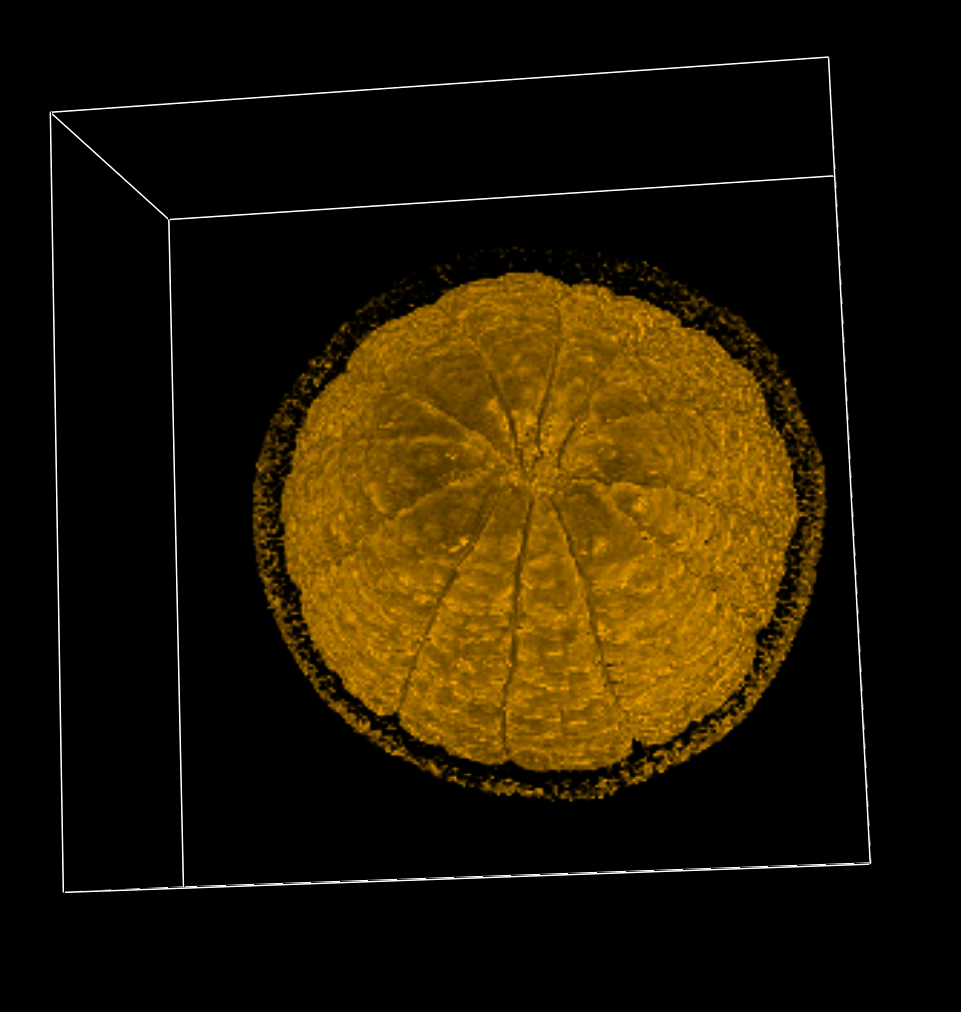
\includegraphics[width=\textwidth]{trilinear-off}
    \caption{Trilinear interpolation disabled.}
  \end{subfigure}
  \hfill
  \begin{subfigure}[b]{0.45\textwidth}
    \centering
    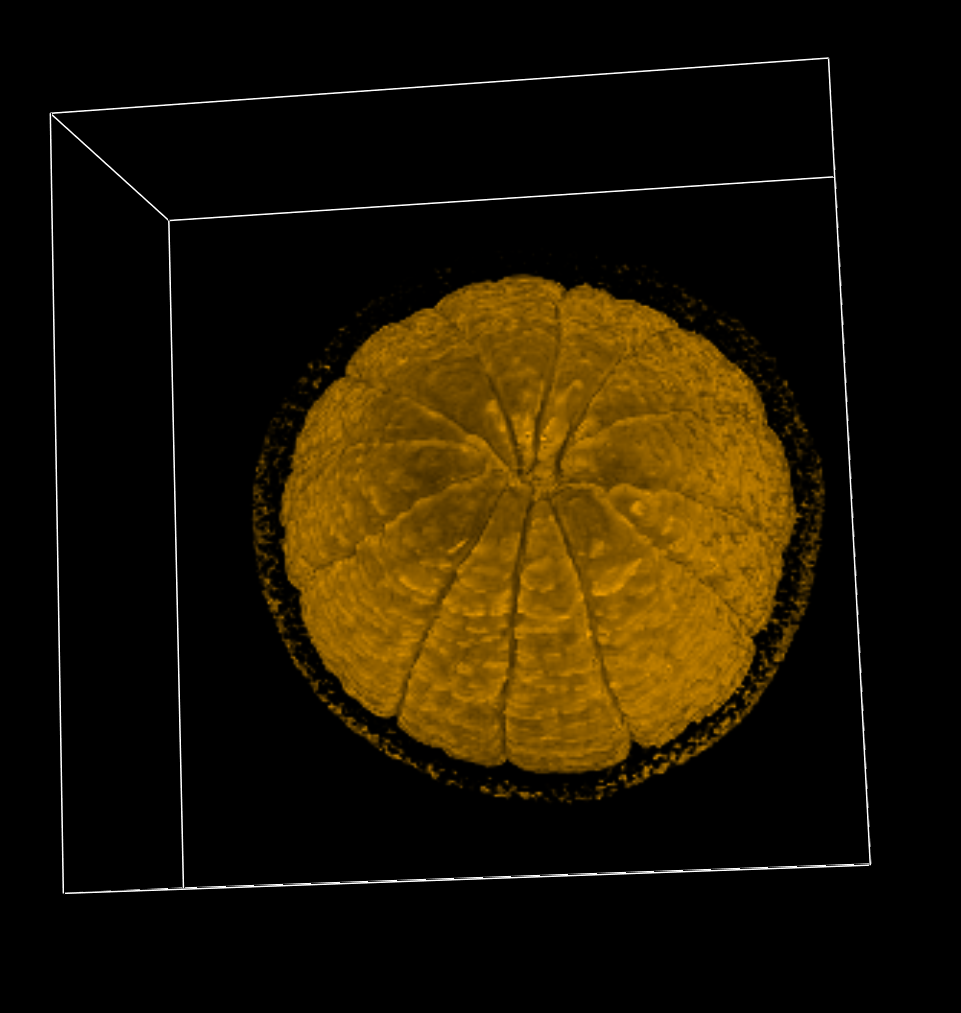
\includegraphics[width=\textwidth]{trilinear-on}
    \caption{Trilinear interpolation enabled.}
  \end{subfigure}
  \caption{Result of compositing visualization with and without trilinear interpolation on the \textit{orange} dataset.}
  \label{fig:trilinear}
\end{figure}

\begin{figure}[h]
  \centering
  \begin{subfigure}[b]{0.45\textwidth}
    \centering
    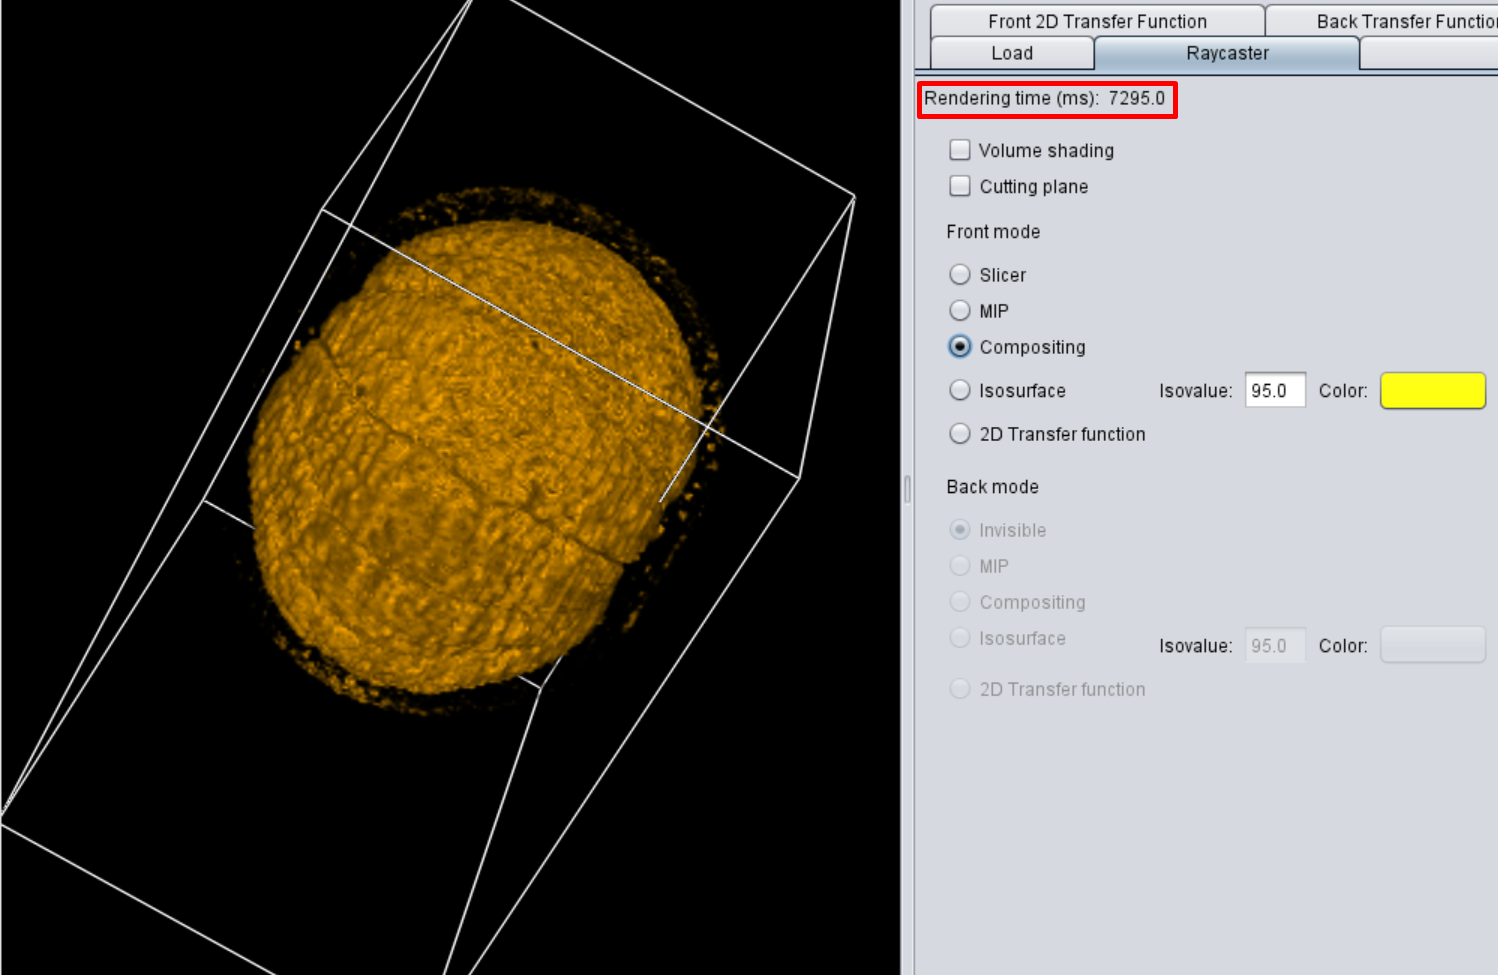
\includegraphics[width=\textwidth]{before-speedup}
    \caption{Interactive mode before speed up changes. Rendering time: 7295 ms }
  \end{subfigure}
  \hfill
  \begin{subfigure}[b]{0.45\textwidth}
    \centering
    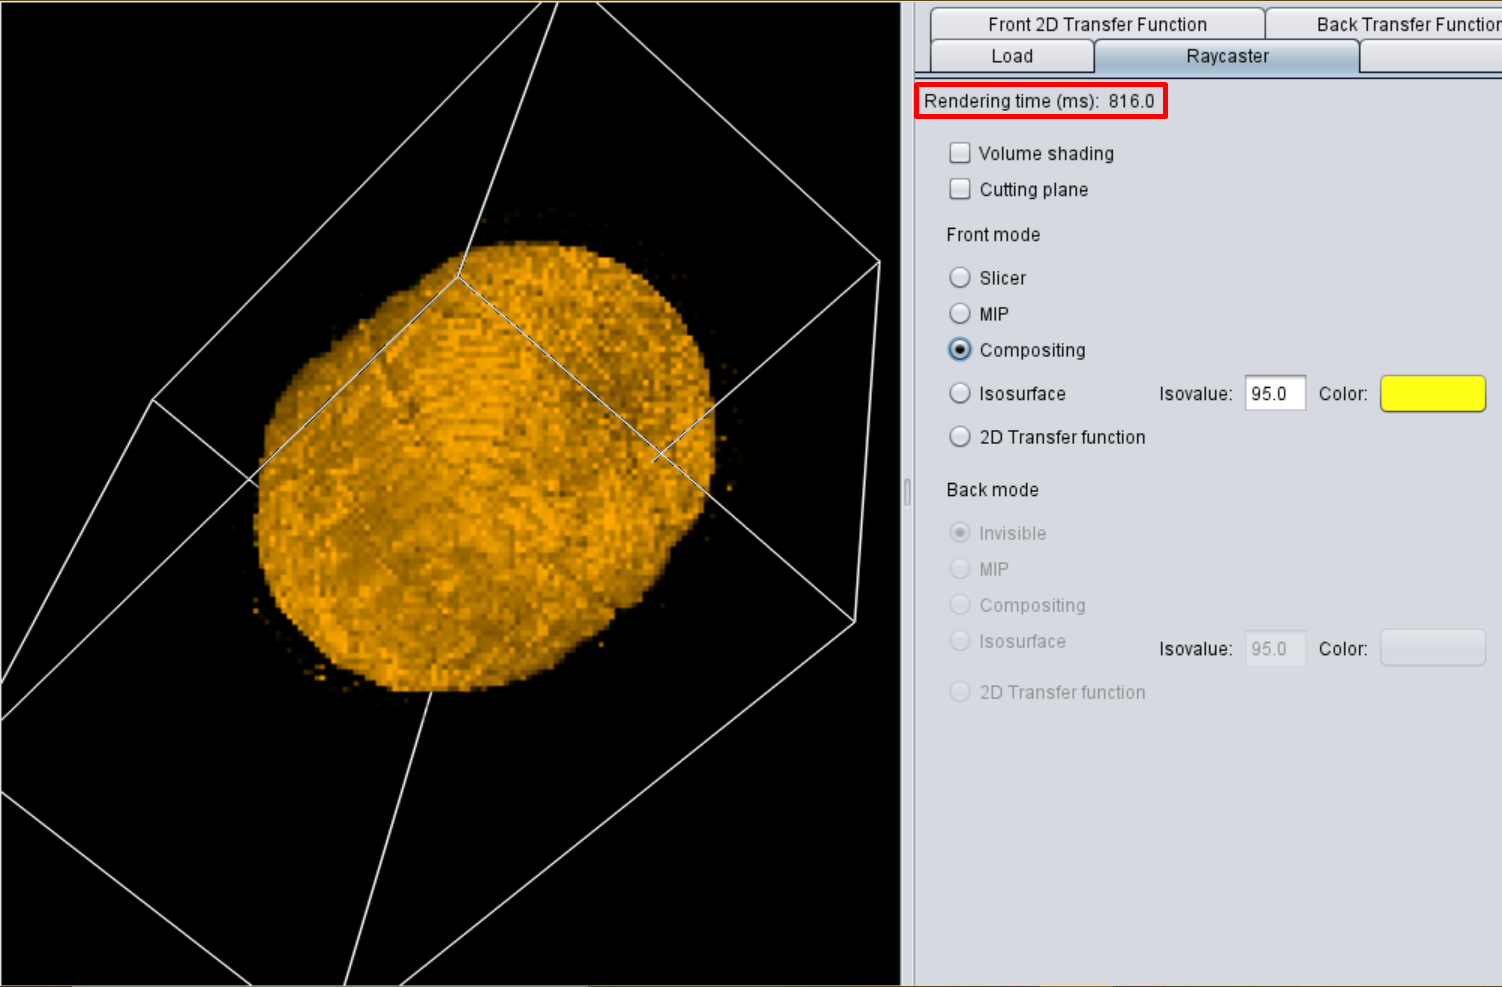
\includegraphics[width=\textwidth]{after-speedup}
    \caption{Interactive mode after speed up changes. Rendering time 816 ms}
  \end{subfigure}
  \caption{Result of speeding up interactive mode on the \textit{orange} dataset.}
  \label{fig:speedup}
\end{figure}

\begin{figure}[h]
  \centering
  \begin{subfigure}[b]{\textwidth}
    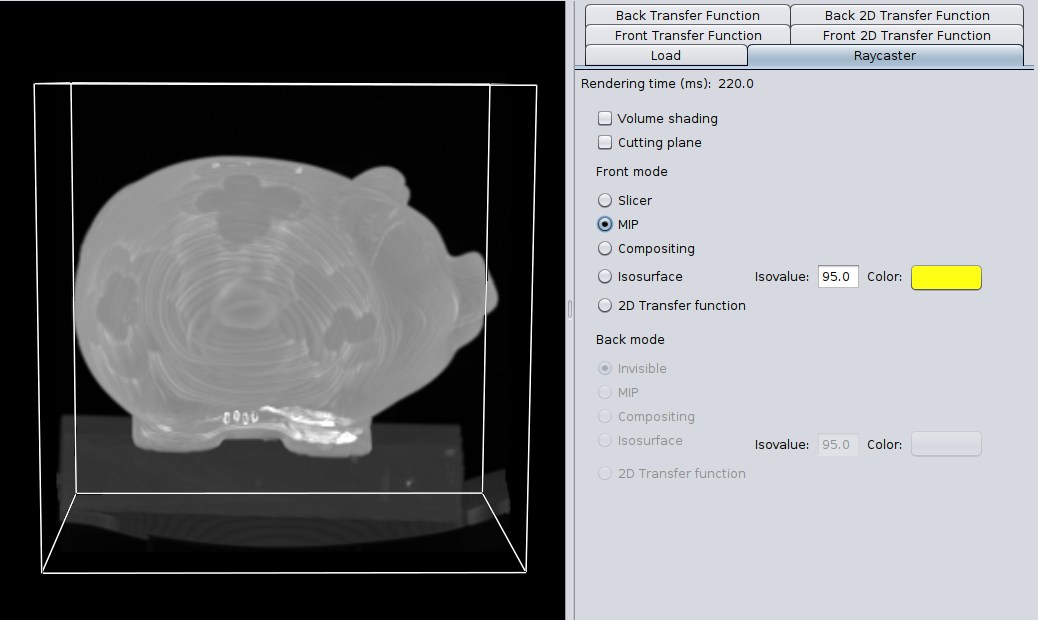
\includegraphics[width=\textwidth]{pig8-mip}
    \caption{MIP conceals the inside of the volume.}
  \end{subfigure}
  \\~\\
  \begin{subfigure}[b]{\textwidth}
    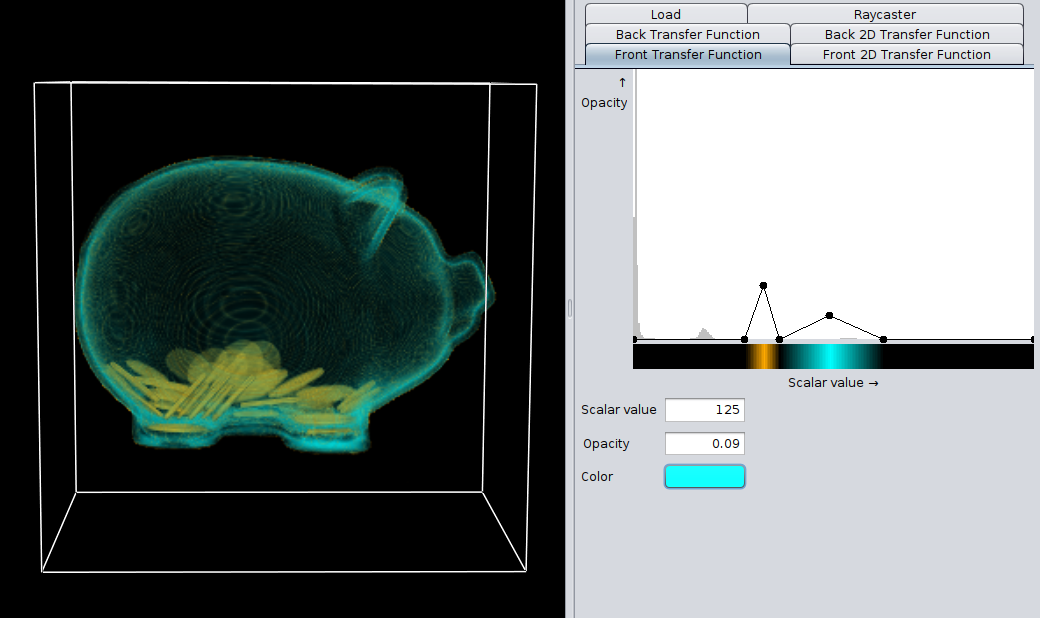
\includegraphics[width=\textwidth]{pig8-composite}
    \caption{Composite rendering highlights two regions of different intensity.}
  \end{subfigure}
  \caption{Comparison of MIP and composite rendering methods on the \textit{pig8} dataset.}
  \label{fig:mipscomp}
\end{figure}

\begin{figure}[h]
  \centering
  \begin{subfigure}[b]{\textwidth}
    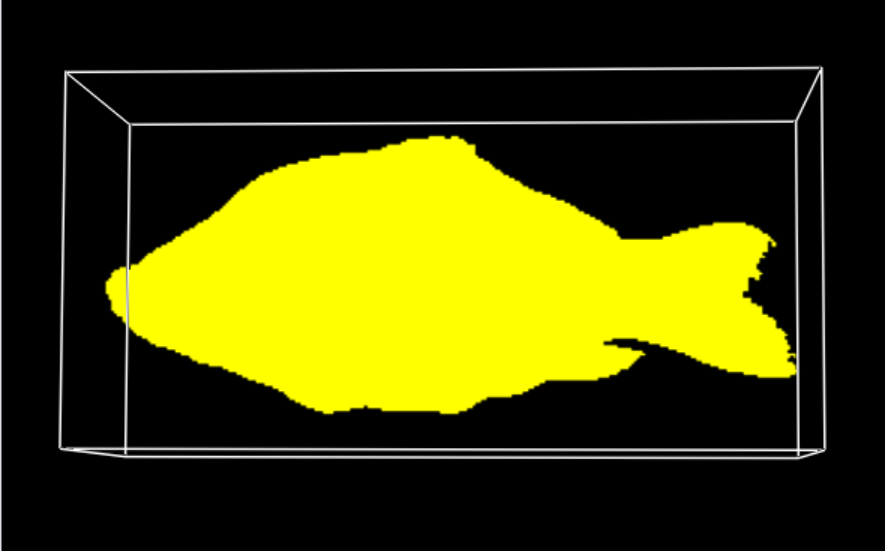
\includegraphics[width=\textwidth]{carp-iso-95}
    \caption{Phong shading disabled.}
  \end{subfigure}
  \\~\\
  \begin{subfigure}[b]{\textwidth}
    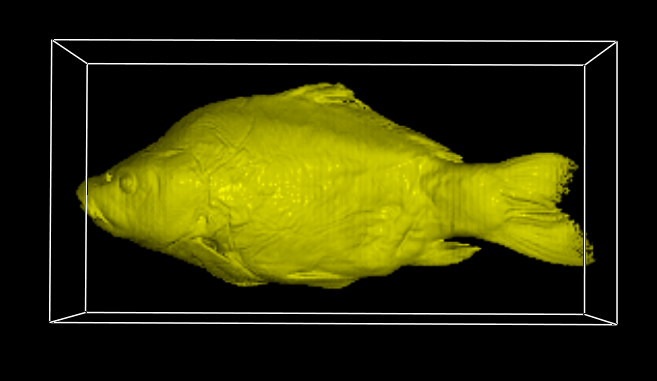
\includegraphics[width=\textwidth]{carp-iso-95-shaded}
    \caption{Phong shading enabled.}
  \end{subfigure}
  \caption{Isosurface raycasting with $C = 95$, with and without shading on the \textit{carp8} dataset.}
  \label{fig:isosurface}
\end{figure}

\begin{figure}[h]
  \centering
  \begin{subfigure}[b]{0.45\textwidth}
    \centering
    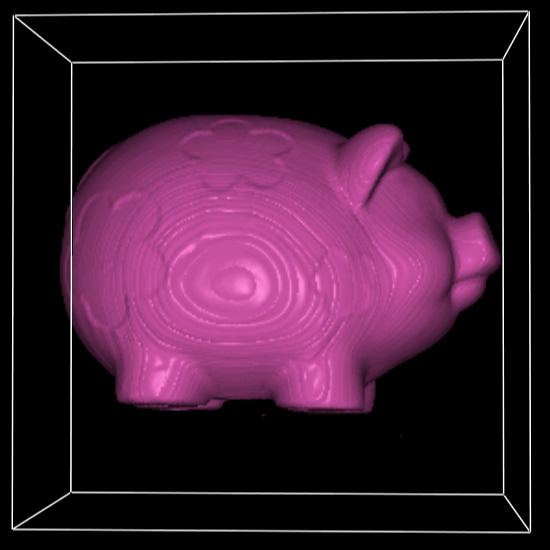
\includegraphics[width=\textwidth]{pig8-phong-default}
    \caption{Default values.}
  \end{subfigure}
  \hfill
  \begin{subfigure}[b]{0.45\textwidth}
    \centering
    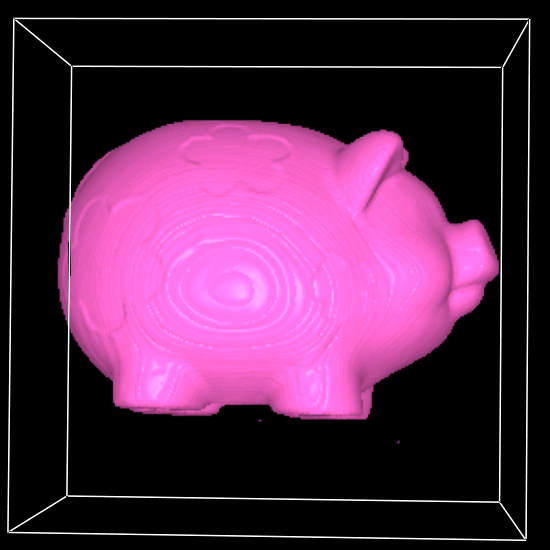
\includegraphics[width=\textwidth]{pig8-phong-ambient05}
    \caption{Ambient $k_a=0.5$, higher than the default.}
  \end{subfigure}
  \\~\\
  \begin{subfigure}[b]{0.45\textwidth}
    \centering
    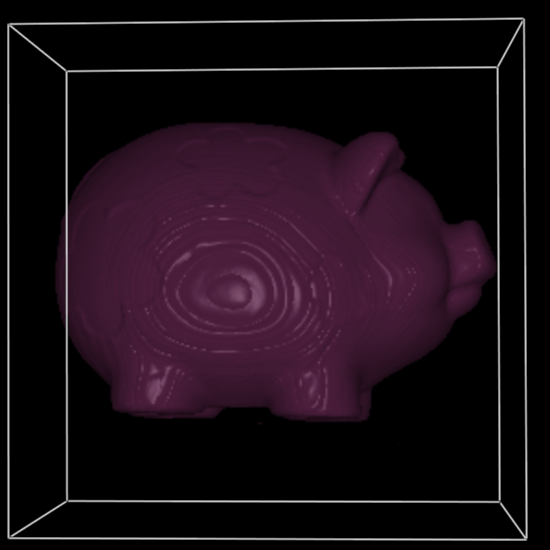
\includegraphics[width=\textwidth]{pig8-phong-diffuse02}
    \caption{Diffuse $k_d=0.2$, lower than the default.}
  \end{subfigure}
  \hfill
  \begin{subfigure}[b]{0.45\textwidth}
    \centering
    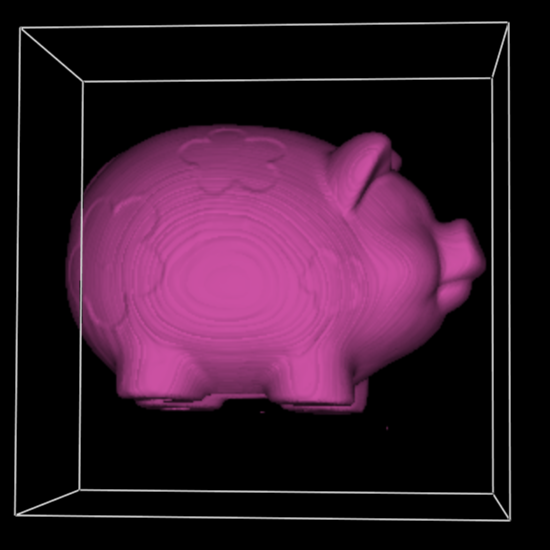
\includegraphics[width=\textwidth]{pig8-phong-specular0}
    \caption{Specular $k_s=0.0$, lower than the default.}
  \end{subfigure}
  \caption{Comparison of the effect of changing different parameters of Phong's shading on \textit{pig8} dataset.}
  \label{fig:phong}
\end{figure}

\begin{figure}[h]
  \centering
  \begin{subfigure}[b]{\textwidth}
    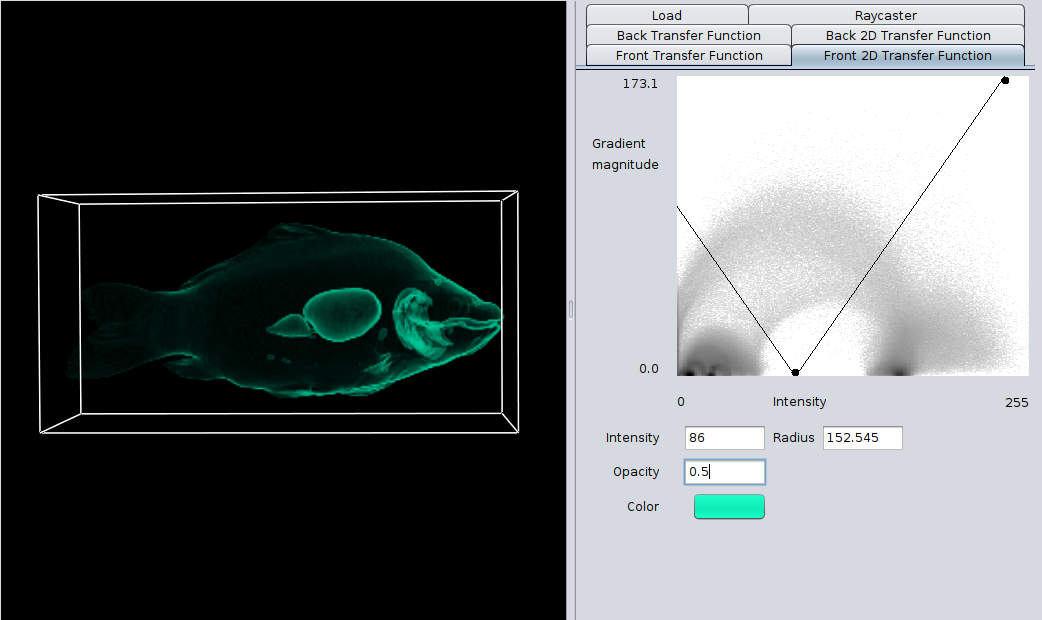
\includegraphics[width=\textwidth]{2dtf}
    \caption{A transfer function revealing lower density features.}
  \end{subfigure}
  \\~\\
  \begin{subfigure}[b]{\textwidth}
    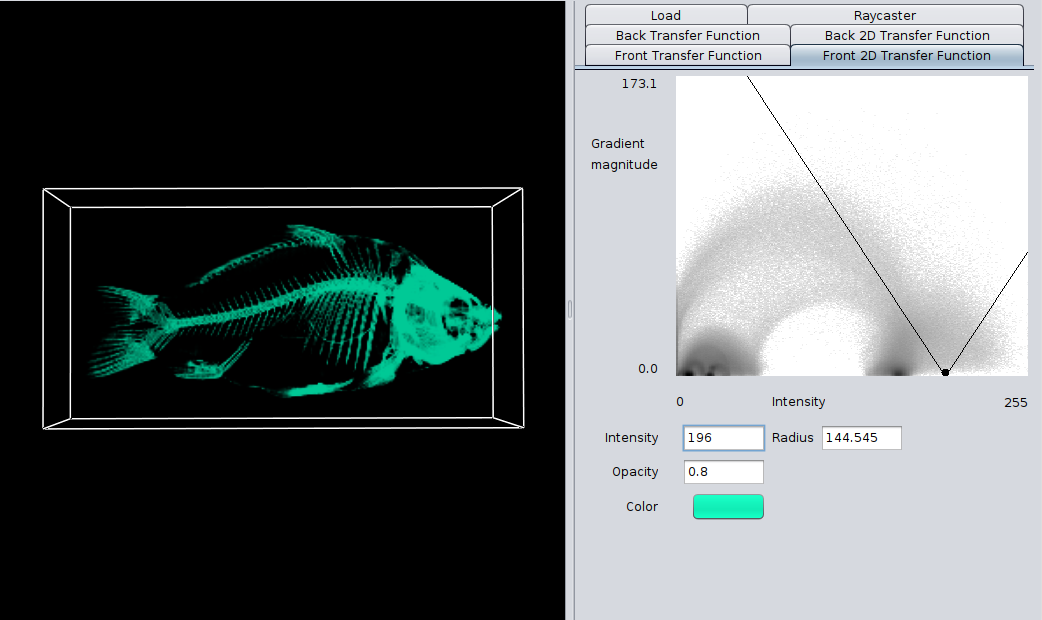
\includegraphics[width=\textwidth]{2dtf-skeleton}
    \caption{A transfer function revealing higher density features.}
  \end{subfigure}
  \caption{Comparison of different 2D transfer functions on \textit{carp8} dataset.}
  \label{fig:2dtf}
\end{figure}

\begin{figure}[h]
  \centering
  \begin{subfigure}[b]{0.45\textwidth}
    \centering
    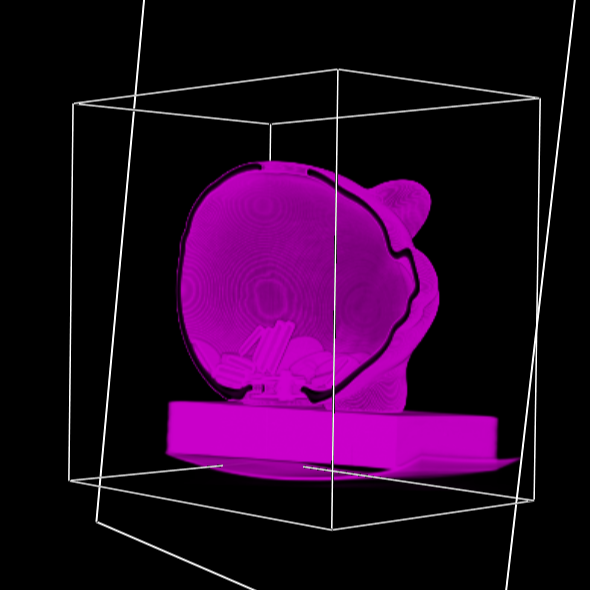
\includegraphics[width=\textwidth]{pig8-cut-plane-coins}
    \caption{The back half rendered with composite, the front half invisble. The inside of the volume is revealed.}
  \end{subfigure}
  \hfill
  \begin{subfigure}[b]{0.45\textwidth}
    \centering
    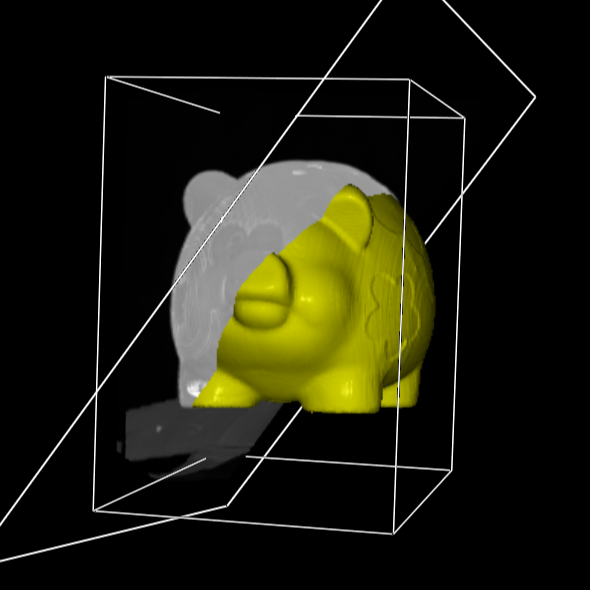
\includegraphics[width=\textwidth]{pig8-cut-plane-renders}
    \caption{MIP and isosurface with shading. Each side of the volume is rendered differently.}
  \end{subfigure}
  \caption{Cutting plane demonstration on the \textit{pig8} dataset.}
  \label{fig:cutplane}
\end{figure}

\begin{figure}[h]
  \centering
  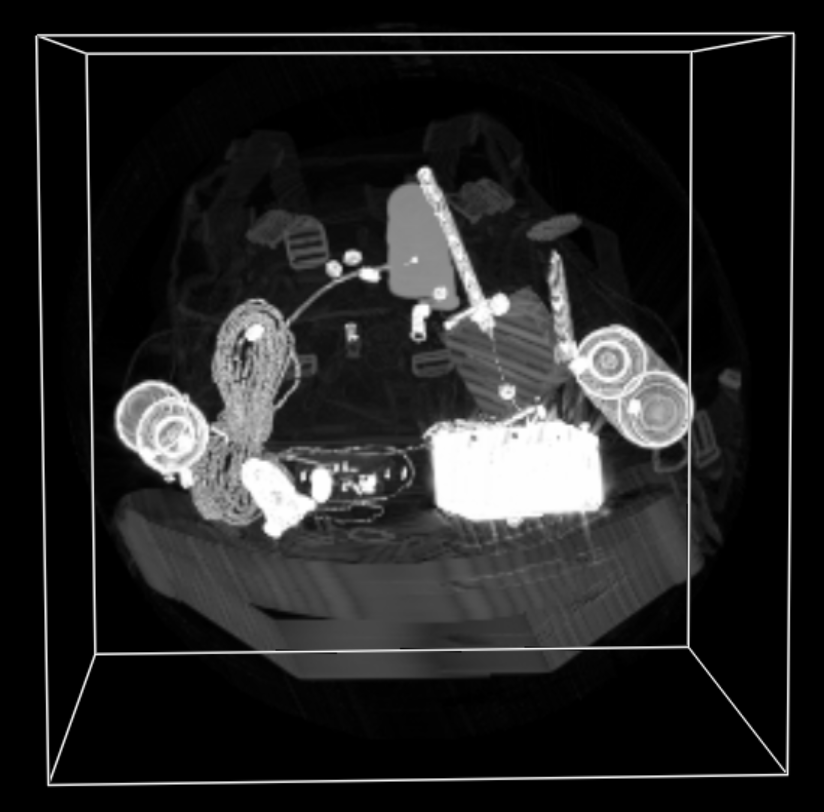
\includegraphics[width=\textwidth]{backpack-MIP}
  \caption{MIP of the \textit{backpack8\_small} dataset, revealing the contents of the backpack.}
  \label{fig:backpack-mip}
\end{figure}

\begin{figure}[h]
  \centering
  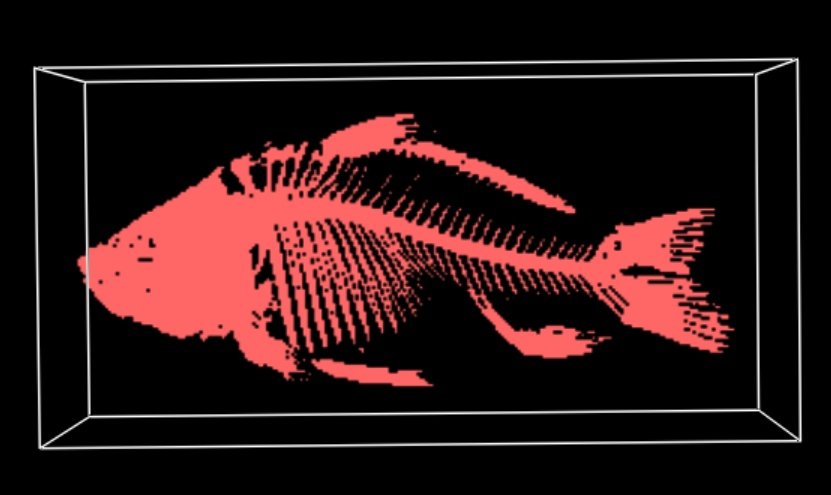
\includegraphics[width=\textwidth]{carp-iso-180}
  \caption{Isosurface raycasting with $C = 180$ on the \textit{carp8} dataset.}
  \label{fig:carp-skelet}
\end{figure}

\begin{figure}[h]
  \centering
  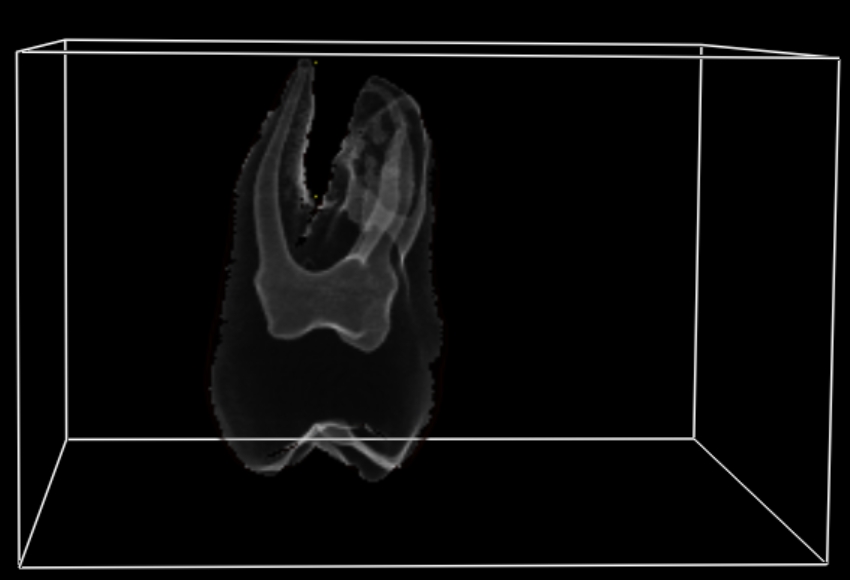
\includegraphics[width=\textwidth]{tooth-2d}
  \caption{The 2D transfer function rendering method on \textit{tooth} dataset with pulp chamber visible. The parameters used are $f_v = 720$, $r = 460$, $\alpha_v = 0.3$.}
  \label{fig:tooth}
\end{figure}

\end{document}
